\documentclass[lettersize,journal]{IEEEtran}
% Packages {{{
\usepackage[ruled,vlined]{algorithm2e}  % psuedocode
\usepackage{amsmath}                    % align, split, ...
\usepackage{amsfonts}                   % \mathbb
\usepackage{balance}                    % final page page column balance
\usepackage{booktabs}                   % nicer tables
\usepackage{cite}                       % \cite
\usepackage{graphicx}                   % \includegraphics[width]{file}
\usepackage{makecell}                   % multi-line cells / better vertical aligning
\usepackage{mathrsfs}                   % \mathscr for E-field (time)
\usepackage{mathtools}                  % \mathclap, \Declare*, aligned
\usepackage{pifont}
\usepackage{stfloats}                   % [b] in \begin{figure}[b]
\usepackage{textcomp}
\usepackage{url}                        % \url{URL} (formatted correctly)
\usepackage{xcolor}                     % for colors
% }}}
% Declared Math Operators / Delimiters {{{
\DeclareRobustCommand{\abs}[1]{\left\lvert #1 \right\rvert}
\DeclareRobustCommand{\norm}[1]{\left\lVert #1 \right\rVert}
\DeclareRobustCommand{\pos}{\vec{r}}
\DeclareRobustCommand{\wavevec}{\mathbf{k}}
\DeclareRobustCommand{\unitWavevec}{\hat{\wavevec}}
\DeclareRobustCommand{\eFreq}{\mathbf{E}}
\DeclareRobustCommand{\hFreq}{\mathbf{H}}
\DeclareRobustCommand{\hank}[2]{H_{#2}^{(#1)}}
\DeclareRobustCommand{\greens}[1]{\mathcal{G}(#1)}
\DeclareRobustCommand{\unitNorm}{\hat{n}}
\DeclareRobustCommand{\bigO}{\mathcal{O}}
\DeclareRobustCommand{\eInc}{\eFreq_i}
\DeclareRobustCommand{\impedanceMat}{\mathbf{Z}}
\DeclareRobustCommand{\innerProd}[2]{\langle #1, #2 \rangle}
\DeclareRobustCommand{\fourier}[1]{\mathcal{F}(#1)}
\DeclareRobustCommand{\fft}[1]{\text{FFT}(#1)}
\DeclareRobustCommand{\ifft}[1]{\text{FFT}^{-1}(#1)}
% }}}
\begin{document}
% Command defs (for .tex readability) {{{
\newcommand{\txSymbol}{T}
\newcommand{\rxSymbol}{R}
\newcommand{\wallSymbol}{S}
\newcommand{\txPos}{\pos_{\txSymbol}}
\newcommand{\rxPos}{\pos_{\rxSymbol}}
\newcommand{\wallPos}{\pos_{\wallSymbol}}
\newcommand{\sourcePower}{P_{\txSymbol}}
\newcommand{\wavenum}{k}
\newcommand{\wallSurf}{S}
\newcommand{\numWallPts}{N_{\wallSurf}}
\newcommand{\numRxPts}{N_{\rxSymbol}}
\newcommand{\eRx}{\eFreq_{\rxSymbol}}
\newcommand{\eWall}{\eFreq_{\wallSurf}}
\newcommand{\hWall}{\hFreq_{\wallSurf}}
\newcommand{\imp}{\eta}
\newcommand{\surfCurrent}{J_{\wallSurf}}
\newcommand{\numBasisFuncs}{N_b}
\newcommand{\coeffs}{\mathbf{a}}
\newcommand{\exciteVec}{\mathbf{V}}
\newcommand{\wallLen}{l_{\text{wall} }}
\newcommand{\rxLen}{l_{\text{Rx} }}
\newcommand{\wavelen}{\lambda}
\newcommand{\meanLength}{\bar{L}}
\newcommand{\defeq}{\overset{\mathclap{\text{def}} }{=}}
\newcommand{\numSurfs}{N_{l}}
\newcommand{\numRays}{N_{\text{rays} }}
\newcommand{\fresnel}{\Gamma}
\newcommand{\curv}{\kappa}
\newcommand{\bigLength}{\check{L}}%{L_{\text{max} }}
\newcommand{\specLen}{l_{\text{spec} }}
\newcommand{\divergenceFactor}{\mathcal{D}}
\newcommand{\incAngles}{N_{\theta_i}}
\newcommand{\scatAngles}{N_{\theta_s}}
\newcommand{\heightFine}{h_{\text{fine}}}
\newcommand{\heightCoarse}{h_{\text{coarse}}}
\newcommand{\heightAging}{h_{\text{aging}}}
\newcommand{\ampFine}{A_{\text{fine}}}
\newcommand{\freqFine}{f_{\text{fine}}}
\newcommand{\ampCoarse}{\langle A_{\text{coarse}} \rangle}
\newcommand{\freqCoarse}{\langle f_{\text{coarse}} \rangle}
% }}}
% Title {{{
\title{Modelling of Diffuse Scattering Effects for Outdoor Ray Tracing}
\author{Andrew Whelan, \emph{Dublin City University}, Prof. Conor Brennan,
        \emph{Dublin City University}}
% The paper headers
\markboth{MEng in Electronic \& Computer Engineering}%
{Shell \MakeLowercase{\textit{et al.}}: Modelling of Diffuse Scattering Effects for
Outdoor Ray Tracing}

\maketitle
% }}}
% Abstract {{{
\begin{abstract}
   Physically accurate outdoor channel modelling for high-frequency systems (e.g.
   5G/6G, LiDAR, SAR) requires robust models for diffuse scattering (DS). Many
   established models, however, are predicated on Gaussian surface statistics. 

   In this paper, we evaluate the performance of several key DS models against a
   numerically exact Method of Moments (MoM) solution in a 2D single-bounce scenario.
   By analyzing surfaces with more realistic, non-Gaussian statistics, we identify
   the specific regimes where these models break down, and offer guidance on the
   selection of the most accurate model for challenging, realistic scattering
   environments.
\end{abstract}
\begin{IEEEkeywords}
Diffuse Scattering, Diffuse Reflection, Channel Model, Ray Tracing, Ray Shooting.
\end{IEEEkeywords}
% }}}
% I.   Introduction {{{
\section{Introduction}
\IEEEPARstart{T}{he} phenomenon of diffuse scattering (DS) is understood to play a
large role in outdoor scenarios, especially at high-frequencies \cite{ref:ER1}.
Figure~\ref{fig:kirchhoff-limit} illustrates the significance of high $\wavenum$ for
a simple indent.

\begin{figure}[!b]
   \begin{center}
      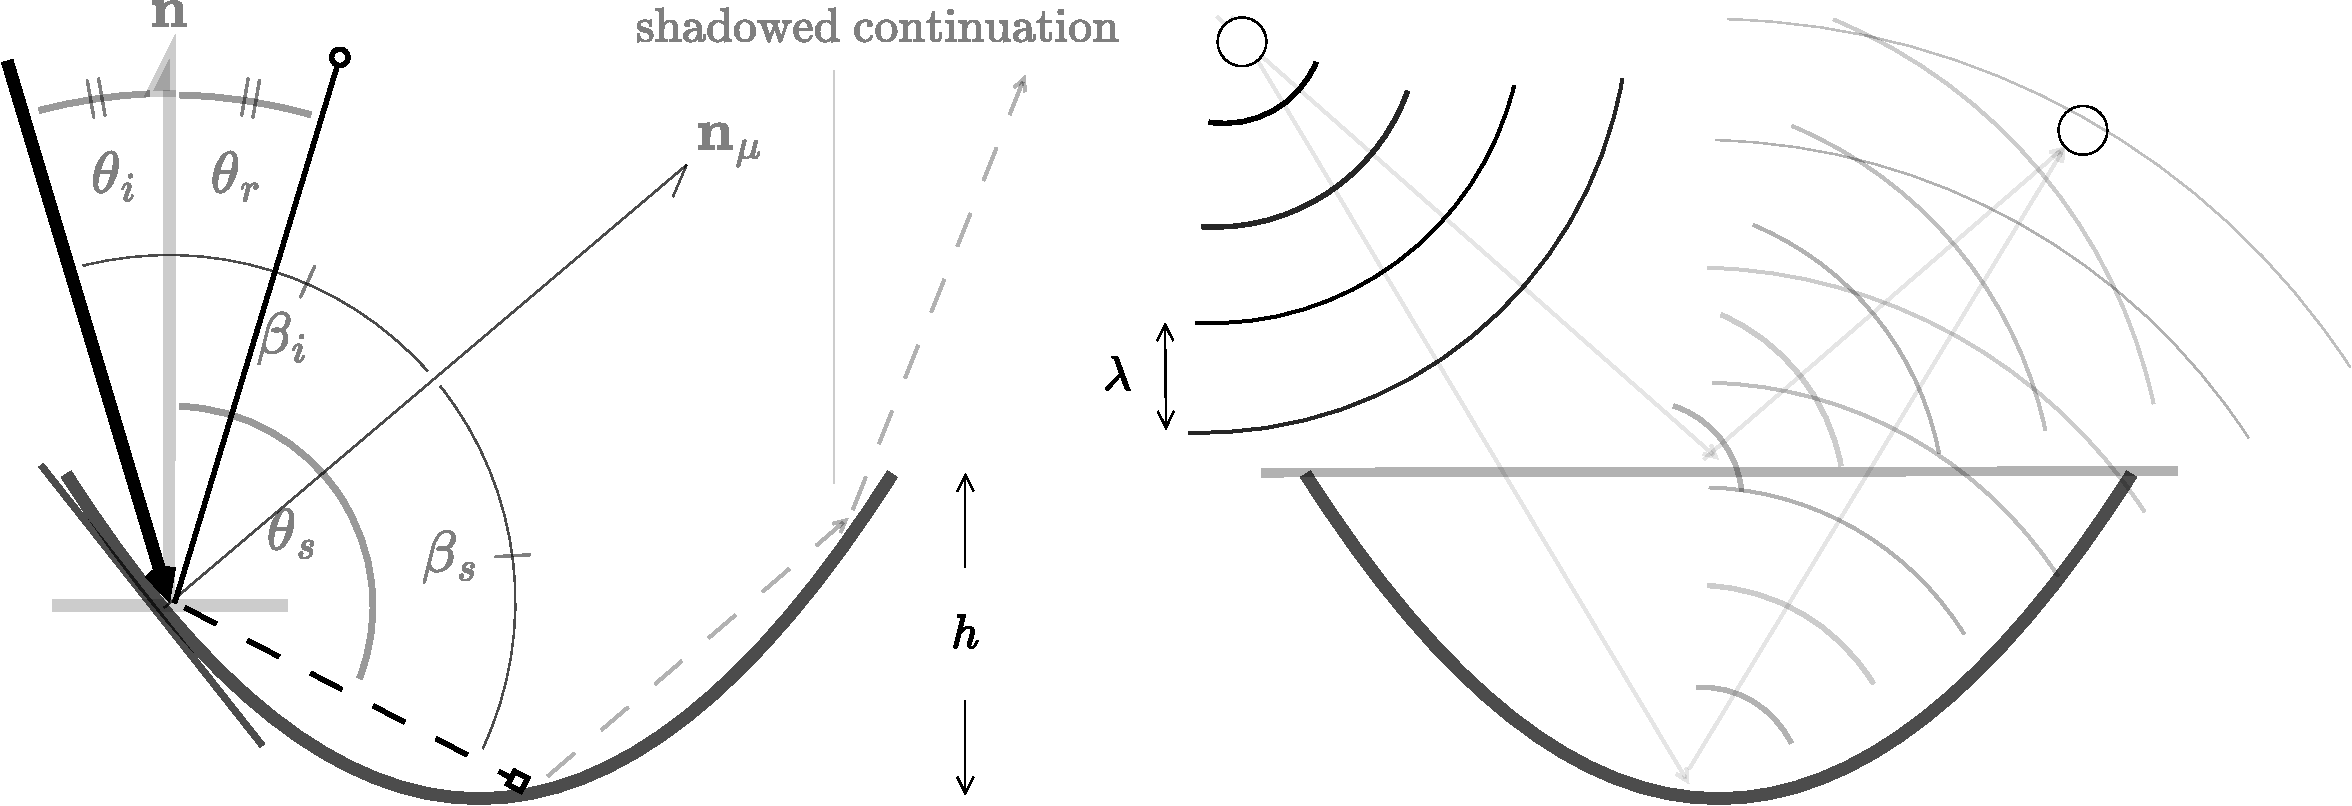
\includegraphics[width=0.46\textwidth]{../figures/kirchhoff-approx-crop.pdf}
   \end{center}
   \caption{A simple indent on a surface (left is the ray POV,  and right is the wave
   POV). When indent depth ($h$) is comparable to, or greater than $\lambda$, as in
   this picture, complex interference becomes non-negligible, and the tangent plane
   approximation fails. This is common for the EHF-UHF range interacting with urban
   features.}\label{fig:kirchhoff-limit}
\end{figure}

A large class of existing models are predicated on Gaussian surface roughness
(statistical models) and/or locally flat tangent planes (e.g. in asymptotic methods)
. Authors in \cite{ref:ER2} identified these as weaknesses when it comes to modelling
diffuse scattering for outdoor surface details. However, a broad comparison between
models is lacking, especially when it comes to modelling the full $\eFreq$-field.
% }}}
% II.  Prior Work {{{
\section{Prior Work}
% TODO: update table, possibly remove appendix... put more models in for comparison
Table~\ref{tab:modelAlgComparison} compares various models in 2d for a fixed point
transmitter, a rough wall, and a line of receivers.
\renewcommand{\arraystretch}{1.5}
\begin{table}[!t]
   \caption{Comparison of Scattering Models 
            (see Appendix~\ref{app:algs})}
   \label{tab:modelAlgComparison}
   \centering
   \begin{tabular}{l l l l}
      \toprule
      Method & Class & Complexity & Limitations \\ 
      \midrule
      \addlinespace MoM & Full-wave & $\bigO( (\wavenum \meanLength )^3)$ &
         \makecell[l]{- Very poor scaling \\ - Requires big mesh} \\
      \addlinespace PO & Asymptotic & $\bigO((\wavenum \meanLength)^2)$ &
         \makecell[l]{- No interscattering \\ - Poor scaling} \\
      \addlinespace GO & Asymptotic & $\bigO(\wavenum \bigLength \log(\wavenum
         \bigLength))$ & \makecell[l]{- No diffuse scattering} \\
      \addlinespace $n$-GO & Asymptotic & $\bigO(n \wavenum \bigLength \log(\wavenum
         \bigLength))$ & \makecell[l]{- No micro-scattering} \\
      \bottomrule
   \end{tabular}
\end{table}
\subsection{Full-Wave Models}
% TODO: update wording for other models... e.g. we mightn't consider all these...
This class of models describes computationally intensive numerical integrations of
the wave equations. The model considered in this work as benchmark is the MoM model
described in Algorithm~\ref{alg:MoM} in Appendix~\ref{app:algs}, and described in
more detail in \cite{ref:Balanis}.
\subsection{Asymptotic Models}
In this class we find models such as the WKB hierarchy \cite{ref:WKB}, PO, and GO
(comprising either ray-shooting (GO-RS) or ray-tracing (GO-RT)) \cite{ref:Balanis}.
Since the WKB method is not widely used for ray-tracers, we only consider PO and GO. 

\subsection{Statistical Models}\label{sec:StatisticalModels}
The prototypical model here is the Beckmann-Kirchhoff family (B-K) described in
\cite{ref:Beckmann}. Here, the average power distribution has an analytical formula.
If a further assumption is made on the phase distribution for diffuse rays, the full
field can be modelled stochastically.

There are also other statistical models of note, including the Integral Equation
Method \cite{ref:IEM}, and the Small Slope Approximation \cite{ref:SSA}, however,
these won't be considered due to their computational infeasibility for ray-tracing.

\subsection{Heuristic Models}
These are a subclass of the Statistical models of section
\ref{sec:StatisticalModels} where, the diffusely scattered power
distribution assumes a fixed parametric form, whose parameters are empirically
matched. These are further divided into models with a single parametric distribution
(e.g. Phong \cite{ref:Phong}, Cook-Torrance \cite{ref:Cook-Torrance}), and models
that use a hybrid of specular and diffuse distributions (e.g. "effective-roughness"
models (ER) described in \cite{ref:ER2}).
% }}}
% III. Model Setup {{{
\section{Model Setup}
\subsection{Ray-Tracing vs. Ray-Shooting}
In order that the models can be compared fairly, it is necessary to choose a
consistent ray-propagation method. There are two broad methods: 
\begin{itemize}
   \item Ray-shooting (RS): rays are propagated from source to receiver, and
   \item Ray-tracing (RT): rays are propagated backward from receiver to source,
      using a path-length minimization algorithm. 
\end{itemize}
A choice in practice is largely dependent on the receiver geometry, with the former
being reserved for wide and continuous receivers. Both types are considered here, but
separately. %TODO: update if not considered...
\subsection{Surface Modelling}
\begin{figure}[!t]
   \begin{center}
      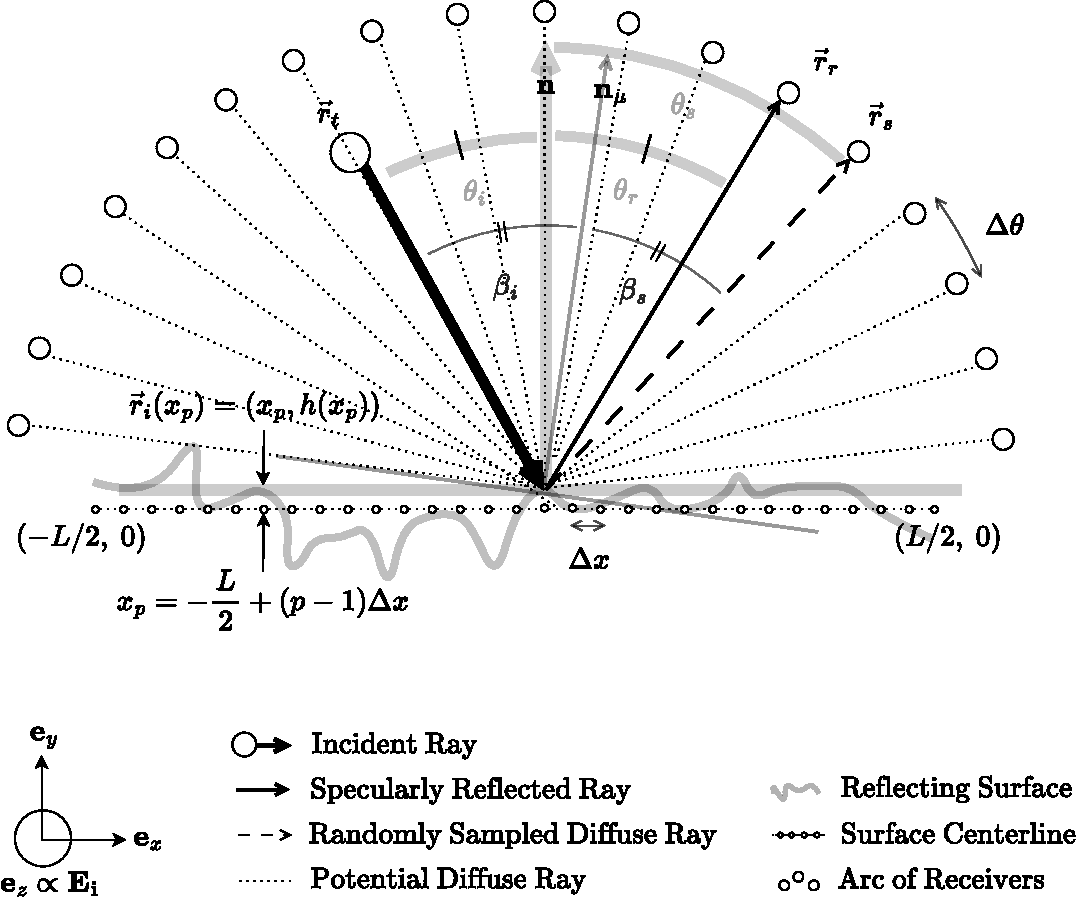
\includegraphics[width=0.45\textwidth]{../figures/setup-geometry-crop.pdf}
   \end{center}
   \caption{Setup Geometry for ray-shooting. The surface tangents, and hence the
   microscopic normal ($\mathbf{n}_{\mu}$), $\beta$ values, and scattering angle
   ($\theta_s$) are assumed apropri unknown. In a stochastic model, the diffuse field
   $\eFreq_s$ is computed for a particular ensemble according to (a) the model's PDF
   for $\theta_s$, and (b) a UID phase $\phi_s$.}\label{fig:setup-geometry}
\end{figure}
The geometric setup is depicted in Figure~\ref{fig:setup-geometry}. Of particular
importance is modelling the surface height $h$. The process for Gaussian
roughness is as follows, following the procedure in \cite{ref:surfaceSimFFT}:
\begin{enumerate}
   \item Specify a Gaussian PDF $f$ with RMS height deviation $\sigma$:
      \begin{subequations}
      \begin{align*} 
         f(h) = \frac{1}{\sigma \sqrt{2 \pi}} e^{-\frac{h^2}{2
            \sigma^2}}
      \end{align*}
      \end{subequations}
   \item Specify a surface correlation function (typically Gaussian, exponential or
      power-law), or equivalently the power-spectral density $S$. A power-law is
      shown here - the Hurst exponent $H$ is a kind of fractal measure :
      \begin{subequations}
      \begin{align*}
         S(k) = |k|^{-(2H+1)}, \quad \text{where } H \in (0,1)
      \end{align*}
      \end{subequations}
   \item Choose a desired discretization of the target height function $h$, and a
      Nyquist determined spacing for $S$:
      \begin{subequations}
      \begin{align*}
         h[x_i], & \text{ with } i \in \{0, \ldots, 2N-1\}, \ \Delta x_i =
            \frac{L}{2N}, \\
         S[k_i], & \text{ with } i \in \{0, \ldots, N\}, \ \Delta k_i =
            \frac{1}{L}
      \end{align*}
      \end{subequations}
   \item Sample $N-1$ UID points $\phi_1, \ldots, \phi_{N-1} \in (0, 2 \pi)$, and one
      $\phi_N \in \{0, \pi\}$ with equal probability, and set
      {
         \small
      \begin{equation*}
         z[k_i] = 
         \begin{dcases*}
            0, & if $i = 0$, \\ 
            \sqrt{S[k_i]} e^{j \phi_i}, & if $1 \leq i \leq N$, \\
            (\sqrt{S[k_{2N-i}]} e^{j \phi_{2N-i}})^*, & if $N+1 \leq i \leq 2N-1$
         \end{dcases*}
         \label{eq:fftSurface}
      \end{equation*}
      }
   \item Perform the IFFT on $z$ to get a surface with the correct properties (apart
      from RMS roughness $\sigma$):
      \begin{equation*}
         h' = \ifft{z}
      \end{equation*}
   \item Rescale $h'$ to have the correct RMS roughness:
      \begin{subequations}
      \begin{align*}
         \sigma' &= \text{STD}(h') \\
         h &= \frac{\sigma}{\sigma'} h'.
      \end{align*}
      \end{subequations}
\end{enumerate}
Generalising this procedure to generate surfaces with a desired non-Gaussian height
profile is required. Authors in \cite{ref:nonGaussianGeneration} generalise to
non-Gaussian PDFs, but here we take an efficient and reasonably realistic approach,
modelling the height of a brick wall as being
\begin{enumerate}
   \item a series of large macro structures $B$ (`bricks') of fixed width $w_B$, and
      with random small tilts $\theta_B \sim N(\mu_{\theta_B}, \sigma_{\theta_B})$,
      with $0 < \mu_{\theta_B}$ small for `lippage' effects,
   \item joined by indents $J$ (`joints') with a super-Gaussian shape (described in
      Figure~\ref{fig:wall-structure}), of random height ($h_J \sim N(\mu_{h_J},
      \sigma_{h_J}$), and width ($w_B \sim N(\mu_{w_J}, \sigma_{w_J})$),
   \item modulated by Gaussian random noise with two separate RMS roughness
      ($\sigma_B, \sigma_J$) and correlation length ($\xi_B, \xi_J$) parameters.
\end{enumerate}
\begin{figure}[!b]
   \begin{center}
      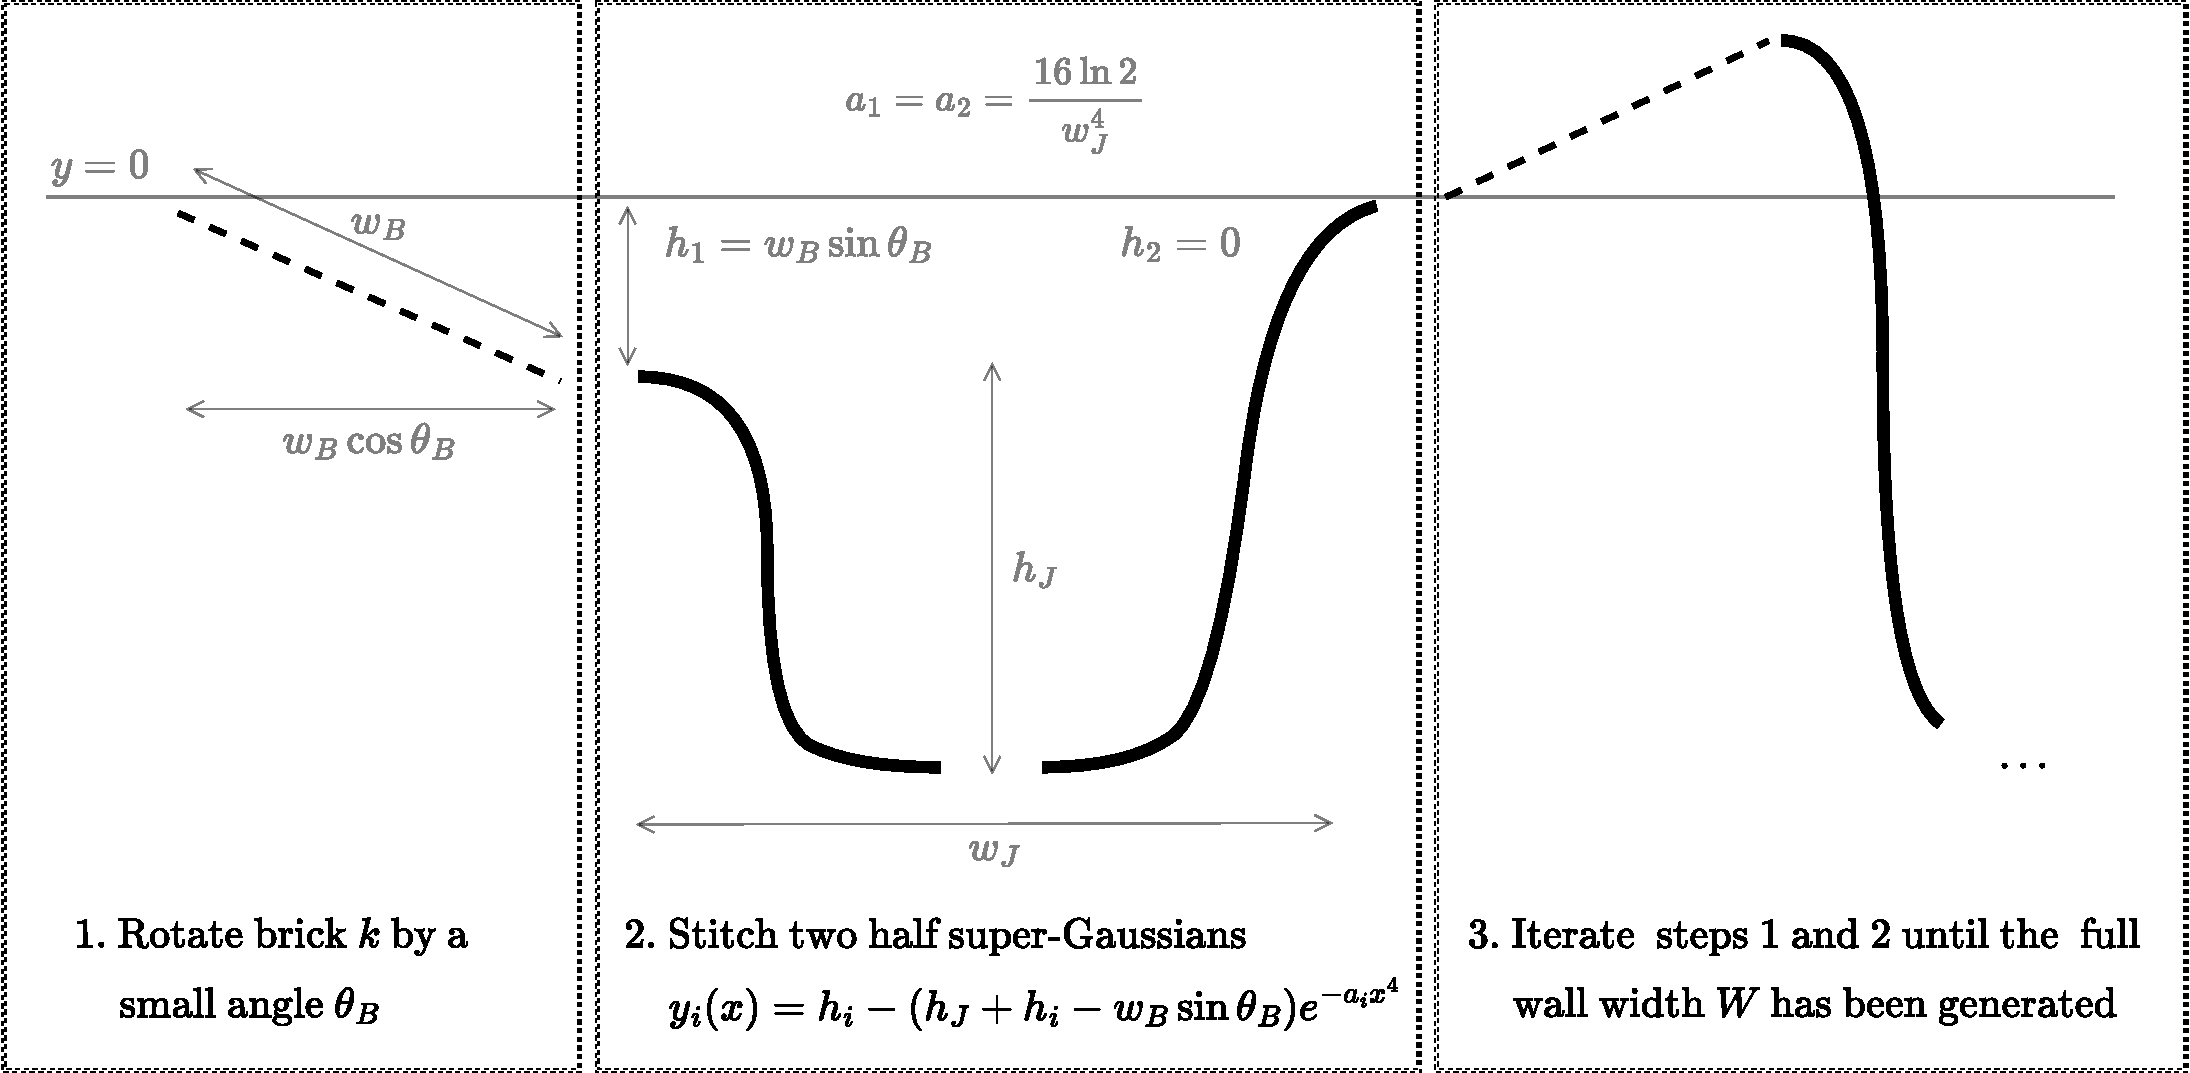
\includegraphics[width=0.48\textwidth]{../figures/wall-structure-crop.pdf}
   \end{center}
   \caption{Base profile for the surface height $h(x)$. The parameters $a_1, a_2$ are
   determined by setting the wall to brick joins to be at the full-width half maximum
   (FWHM).}\label{fig:wall-structure}
\end{figure}

to:
\begin{enumerate}
   \item fine manufacturing processes (subtractive),
   \item coarse manufacturing processes (additive), and
   \item aging defects (subtractive).
\end{enumerate}
Non-Gaussian variations are due to skewness in the individual variations, and are
modelled by applying a hyperbolic tangent to the Gaussian preprocessed functions. The
result of this process is shown in Figure~\ref{fig:surfaceHeight}.
\begin{figure}[!b]
   \begin{center}
      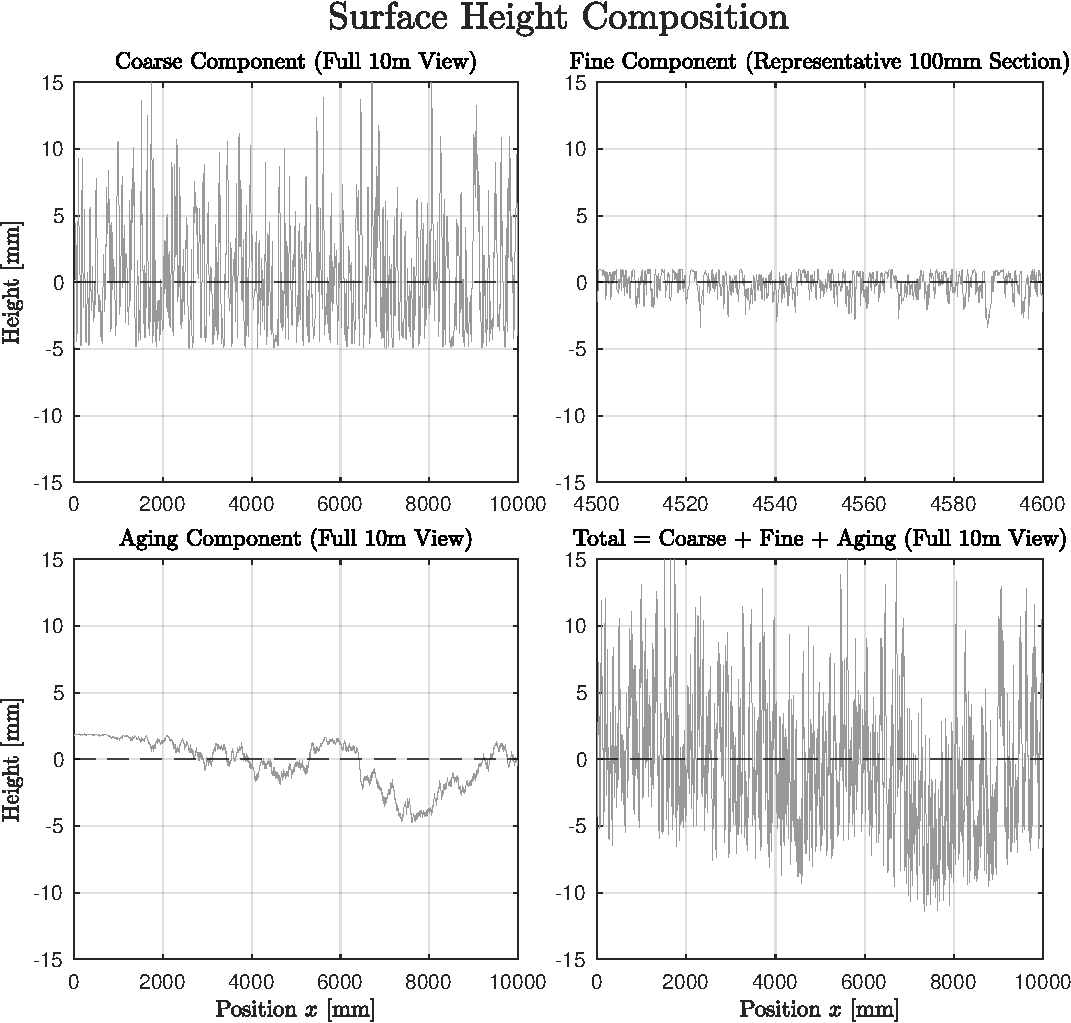
\includegraphics[width=0.47\textwidth]{../figures/surfaceHeight-crop.pdf}
   \end{center}
   \caption{$h = h_{\text{coarse}} + h_{\text{fine}} + h_{\text{aging}}$.}\label{fig:surfaceHeight}
\end{figure}


The height function is therefore considered as a compound of three terms:
\setcounter{equation}{0}
\begin{equation}
   h = \heightCoarse + \heightFine + \heightAging,
      \label{eq:heightModel}
\end{equation}
%\begin{figure}[!b]
%   \begin{center}
%      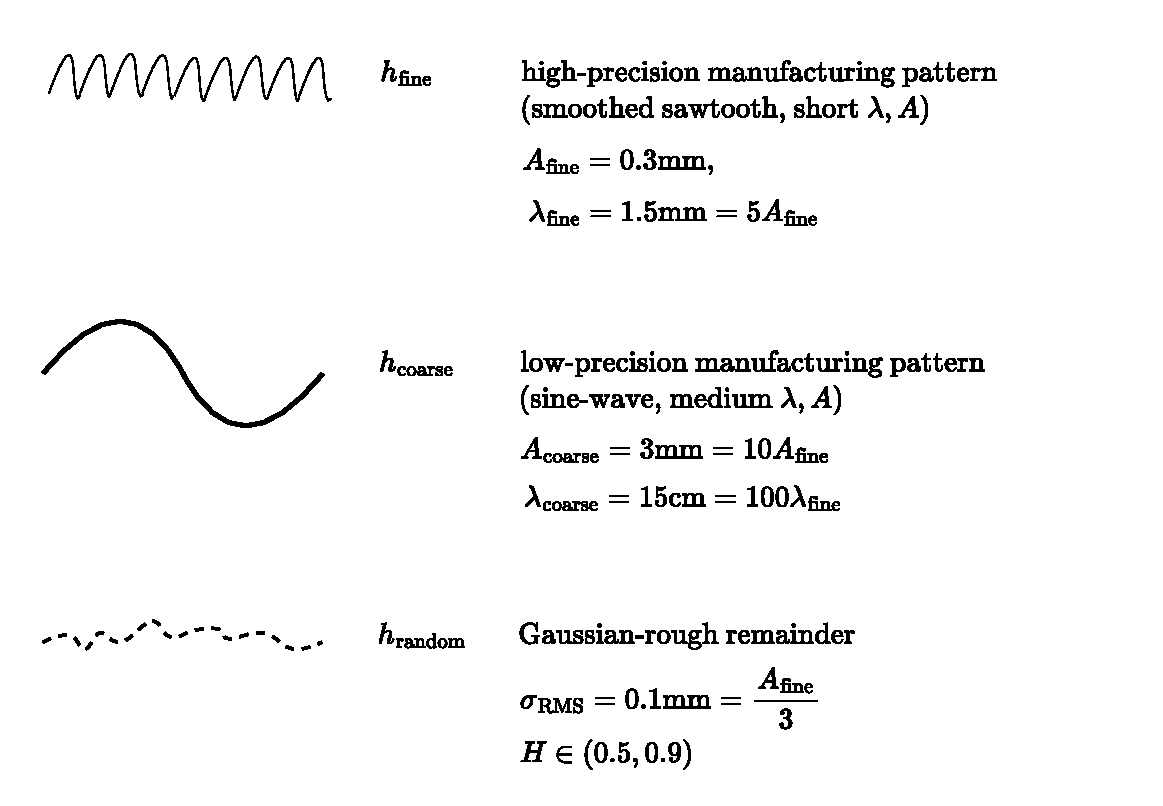
\includegraphics[width=0.55\textwidth]{../figures/heightDecomp.pdf}
%   \end{center}
%   \caption{Semi-realistic height decomposition. The random component can be modelled
%   as described above, where $H$ is the Hurst exponent. The sawtooth wave is smoothed
%   by using a low pass filter.}\label{fig:heightDecomp}
%\end{figure}
where each stage is preprocessed as a Gaussian rough surface, with postprocessing by
a hyperbolic tangent and with defined RMS roughness:
\begin{itemize}
   \item $\heightCoarse$ is preprocessed with exponential
      PSD, with correlation length $l_{\text{coarse}} = 50\text{mm}$, and
      postprocessed with RMS roughness $\sigma_{\text{coarse}} = 5\text{mm}$,
   \item $\heightFine$ is preprocessed with Gaussian PSD,
      with correlation length $l_{\text{fine}} = 1\text{mm}$, and postprocessed with
      RMS roughness $\sigma_{\text{fine}} = 1 \text{mm}$, and 
   \item $\heightAging$ is preprocessed with power law PSD, with Hurst exponent
      $H=0.5$, and postprocessed with RMS roughness $\sigma_{\text{aging}} = 2
      \text{mm}$.
\end{itemize}
% }}}
\subsection{Antenna Placement}
A microcell scenario is considered. Here, the source is within a radius small enough
that the curvature of the incoming wave cannot be neglected. We therefore choose a
cylindrical incoming wave source at a distance 20m from the wall center, and a
semi-circle of receiver antennas within a 25m distance to the wall center:
\begin{subequations}
\begin{align}
   \txPos &= \begin{bmatrix} - 10 \sqrt{2} \\ 10 \sqrt{2} \end{bmatrix} =
      20 \begin{bmatrix} - \cos\frac{\pi}{4} 
      \\ \sin\frac{\pi}{4} \end{bmatrix} \\ 
   \rxPos &= \begin{bmatrix} - 25 \cos\theta_s \\ 25 \sin\theta_s \end{bmatrix},
      \text{ where } \theta_s \in \left(-\frac{\pi}{2}, \frac{\pi}{2}\right).
\end{align}
\end{subequations}


\subsection{Models Used}
\subsubsection{MoM Benchmark}
MoM is used as a benchmark model. The basis functions used are a 1D equivalent of the
Rao-Wilton-Glisson (RWG) basis functions \cite{ref:RWGBasis}, which are essentially
shifted, overlapping triangular `hats', defined on each node in the arclength domain
as $1$ on this node, decreasing uniformly to 0 on either side.

\subsubsection{Microfacet ($\mu$-facet)}
This model assumes the following (see Figure~\ref{fig:microfacet})
\begin{itemize}
   \item Gaussian randomly-distributed surface-slopes,
   \item Locally specular ray behaviour,
   \item Uniformly randomly distributed reflected phase,
   \item Smith masking/shadowing geometric factor \cite{ref:geometricMasking}
\end{itemize} 

\begin{figure}
   \begin{center}
      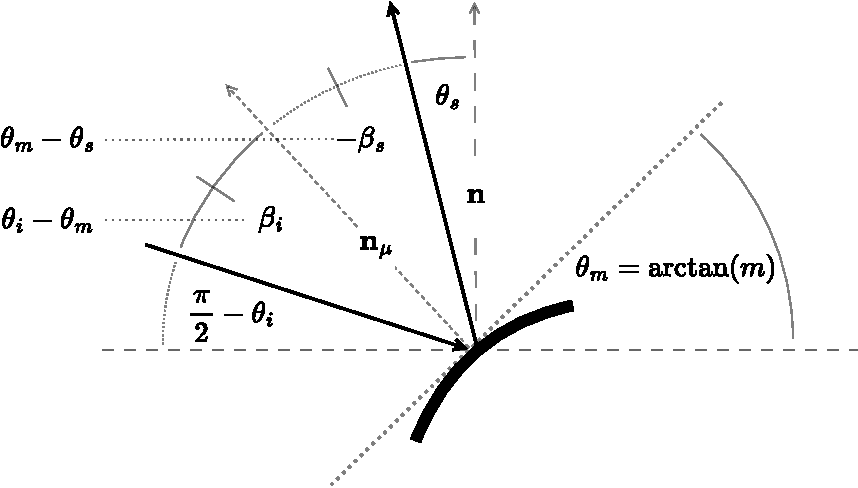
\includegraphics[width=0.40\textwidth]{../figures/microfacet-crop.pdf}
   \end{center}
   \caption{$\mu$-facet model geometry. The diagram implies that $m = \tan \left(
   \frac{\theta_i + \theta_s}{2} \right)$. The scattering angle PDF
   $f_{\Theta_s}(\theta_s)$ can be derived from this as $f_{\Theta_s}(\theta_s) = f_M
   (m(\theta_s)) \left\lvert \frac{dm}{d \theta_s} \right \rvert$, where $f_M(m) =
   \frac{1}{\sqrt{2 \pi} \sigma} e^{- \frac{m^2}{2 \sigma^2}} $ is the PDF for
   surface slopes. The Fresnel coefficients $\fresnel$ are computed with respect to
   $\beta_i = \frac{\theta_i - \theta_s}{2}$}\label{fig:microfacet}
\end{figure}

%\begin{subequations}
%\begin{align}
%   \Lambda_n(l) &= 
%      \begin{cases} 
%         \frac{l - l_{n-1}}{L_{n-1}} & \text{for } l \in [l_{n-1}, l_n] \\ 
%         \frac{l_{n+1} - l}{L_n} & \text{for } l \in [l_n, l_{n+1}] \\ 
%         0 & \text{otherwise, where}
%      \end{cases} \\
%   $l_n$
%\end{align}
%\end{subequations}

\newpage
\appendices
% Appendix A: Algorithms {{{
\section{Algorithms}\label{app:algs}
For all of the below, we can obtain estimates of the numerical parameters (various
$N$) in terms of geometrical ($\wallLen$, $\rxLen$, $\meanLength$) and wave (wavenumber
$\wavenum$) parameters by
\begin{enumerate}
   \item Choosing spacing $\Delta x = \frac{\wavelen}{10}$ for points along the wall,
   \item Choosing spacing $\Delta x = \frac{\wavelen}{2}$ for points along the
      receiver (Nyquist criterion),
   \item Converting to $\Delta x \to N, l$ by using $\Delta x = \frac{l}{N}$,
   \item Converting $\wavelen$ to $\wavenum$ by using $\wavelen = \frac{2
      \pi}{\wavenum}$, and
   \item (Optionally) use the GM length $\meanLength \defeq
      \sqrt[\numSurfs]{(\prod_{i=1}^{\numSurfs} l_i)}$, or in the case of $\log$
      factors, use the maximum dimension $\bigLength \defeq \max_{i=1}^{\numSurfs}
      l_i$
\end{enumerate}

\begin{algorithm}[!h]
\footnotesize
\SetAlgoLined
\caption{Method of Moments (MoM) \\
         \hspace*{2cm} $\bigO((\wavenum \cdot \meanLength)^3) = \bigO\left(
         \left(\frac{5}{\pi}\right)^3 \cdot \wavenum^3 \cdot \wallLen^3 \right)$ \\
         \hspace*{2cm} $= \bigO(\numBasisFuncs^3) = \bigO(\numBasisFuncs^2 +
         \numBasisFuncs^3 + \numBasisFuncs \cdot \numRxPts)$}\label{alg:MoM}
\For{$m \leftarrow 1$ \KwTo $\numBasisFuncs$}{
   $\exciteVec_m \leftarrow \innerProd{\eInc(\txPos)}{g_m}$\;
   \For{$n \leftarrow 1$ \KwTo $\numBasisFuncs$}{
      $\impedanceMat_{mn} \leftarrow \innerProd{\mathcal{L}(f_n)}{g_m}$\;
   }
}
\BlankLine

Solve $\impedanceMat \coeffs = \exciteVec$ for the unknown current coefficients $\coeffs$\;
\BlankLine

\For{$\numRxPts$ points $\rxPos$ on receiver}{
   $\eRx ( \rxPos ) \leftarrow 0$\;
   \For{$n \leftarrow 1$ \KwTo $\numBasisFuncs$}{
      $\eRx( \rxPos ) \leftarrow \eRx( \rxPos) + \coeffs_n \cdot \mathcal{L}(f_n)(\rxPos)$\;
   }
}
\KwRet{$\coeffs, \eRx$}
\end{algorithm}

\begin{algorithm}[!h]
\footnotesize
\SetAlgoLined
\caption{Physical Optics (PO) \\
         \hspace*{2cm} $\bigO((\wavenum \cdot \meanLength)^2) = \bigO
         \left(\frac{5}{\pi^2} \cdot \wavenum^2 \cdot \wallLen \cdot \rxLen \right)$
         \\
         \hspace*{2cm} $= \bigO(\numWallPts \cdot \numRxPts) = \bigO(\numWallPts +
         \numWallPts \cdot \numRxPts)$}\label{alg:PO}
\For{$\numWallPts$ points $\wallPos$ on the wall}{
   $\unitNorm(\wallPos) \leftarrow \text{normal}(\wallPos)$\;
   $\eWall(\wallPos) \leftarrow \sqrt{\frac{\sourcePower \imp \wavenum}{2}}
      \greens{\wavenum \norm{\wallPos - \txPos}} \unitWavevec$\;
   $\hWall(\wallPos) \leftarrow - \frac{j}{\imp \wavenum} \nabla \times \eWall$\;
   $\surfCurrent(\wallPos) \leftarrow 2 \unitNorm \times \hWall$\;
}
\BlankLine
\For{$\numRxPts$ points $\rxPos$ on receiver}{
   $\eRx ( \rxPos ) \leftarrow 0$\;
   \For{$\numWallPts$ points $\wallPos$ on the wall}{
      $\eRx( \rxPos ) \leftarrow \eRx( \rxPos) + \Delta_{\wallSurf} \greens{\wavenum \norm{\rxPos -
      \wallPos}} \surfCurrent(\wallPos)$\;
   }
   $\eRx( \rxPos ) \leftarrow -\frac{\wavenum \imp}{4} \eRx$\;
}
\KwRet{$\eRx$}
\end{algorithm}

\begin{algorithm}[!h]
\footnotesize % Using \small to match the others, not \footnotesize
\SetAlgoLined
\caption{Geo. Optics -- Ray Shooting (GO-RS) \\
         \hspace*{2cm} $\bigO(\numRays \cdot \log(\numWallPts))$}\label{alg:GO-RS}

\For{$n \leftarrow 1$ \KwTo $\numRays$}{
   Generate initial ray $(\unitWavevec_i, E_0)$ from source $\txPos$\;
   \BlankLine

   %--- Propagate to wall and reflect ---
   $\wallPos \leftarrow \text{find\_intersection}(\unitWavevec_i, \txPos, \text{mesh}_{\wallSurf})$\;
   \If{no intersection}{
      continue\;
   }
   $\unitNorm \leftarrow \text{get\_normal}(\wallPos)$\;
   \If{ray hits from behind}{
      continue\;
   }
   $\unitWavevec_r \leftarrow \text{reflect}(\unitWavevec_i, \unitNorm)$\;
   \BlankLine
   
   %--- Propagate to receiver and accumulate field ---
   $\rxPos \leftarrow \text{find\_intersection}(\unitWavevec_r, \wallPos, \text{mesh}_{R})$\;
   \If{no intersection}{
      continue\;
   }
   $\fresnel \leftarrow \text{fresnel\_coefficient}(\unitWavevec_i, \unitNorm)$\;
   $\divergenceFactor \leftarrow \text{divergence}(\txPos, \wallPos, \rxPos, \text{curvatures})$\;
   $\text{pathLen} \leftarrow \norm{\wallPos - \txPos} + \norm{\rxPos - \wallPos}$\;
   
   $\eRx(\rxPos) \leftarrow \eRx(\rxPos) + E_0 \cdot \fresnel \cdot \divergenceFactor \cdot e^{j \wavenum \cdot \text{pathLen}}$\;
}
\KwRet{$\eRx$}
\end{algorithm}

\begin{algorithm}[!h]
   \footnotesize
   \SetAlgoLined
   \caption{Beckmann-Kirchhoff (B-K) \\
            \hspace*{2cm} $\bigO() = \bigO()$ \\
            \hspace*{2cm} $= \bigO() = \bigO()$}\label{alg:BK}
   \For{$n \leftarrow 1$ \KwTo $N$}{
   %--- Step 1: Generate a valid interaction path ---
   $(\text{path\_found}, \txPos, \wallPos, \rxPos, \text{weight}) \leftarrow
   \text{generate\_path}(\text{method})$\;
   \If{not path\_found}{
      continue\;
   }
   \BlankLine
   
   %--- Step 2: Evaluate the physical contribution of this path ---
   $\theta_i \leftarrow \text{calc\_angle}(\txPos, \wallPos, \text{normal}(\wallPos))$\;
   $\theta_s \leftarrow \text{calc\_angle}(\rxPos, \wallPos, \text{normal}(\wallPos))$\;
   $\fresnel \leftarrow \text{fresnel\_coefficient}(\theta_i, \eta_r)$\;
   % F is a function of R, angles, polarization, etc.
   $F \leftarrow \text{scattering\_factor}(\theta_i, \theta_s, \fresnel)$\; 
   $\text{pathLen} \leftarrow \norm{\wallPos - \txPos} + \norm{\rxPos - \wallPos}$\;
   \BlankLine

   %--- Step 3: Calculate the field contribution and apply weight ---
   $E_{path} \leftarrow \frac{E_0}{\text{pathLen}} \cdot F \cdot e^{j k \cdot \text{pathLen}}$\;
   $E_{final\_contrib} \leftarrow E_{path} \cdot \text{weight}$\;
   
   %--- Step 4: Accumulate the result ---
   $E_{diff}(\rxPos) \leftarrow E_{diff}(\rxPos) + E_{final\_contrib}$\;
}

\For{each $R$ in $R_{set}$}{
   $E_{diff}(R) \leftarrow \frac{1}{N} E_{diff}(R)$\;
}
\KwRet{$E_{diff}$}
\end{algorithm}

%\begin{algorithm}[!h]
%\footnotesize
%\SetAlgoLined
%\caption{Beckmann-Kirchhoff (B-K) Model \\
%         \hspace*{2cm} $\bigO(N_\theta)$ for one incident angle}\label{alg:KB}
%% Define the inputs
%\KwIn{RMS Roughness $\sigma$, Correlation Length $\xi$}
%\KwIn{Impedance $\eta$, Wavenumber $k$}
%\BlankLine
%
%\For{$\incAngles$ incident angles $\theta_i \in (-\frac{\pi}{2}, \frac{\pi}{2})$}{
%   Generate initial ray $(\unitWavevec_i, E_0)$ from source $\txPos$\;
%   $P_i \leftarrow \text{incident\_power}(\unitWavevec_i, E_0, \eta, S)$\;
%   $\fresnel \leftarrow \text{fresnel\_coefficient}(\theta_i, \eta)$\;
%   $P_r = \abs{\fresnel}^2 P_i $\;
%   $g = (2 \wavenum \sigma \cos \theta_i )^2$\;
%   $P_{\text{coherent}} \leftarrow  e^{-g} P_r$\;
%   $P_{\text{incoherent}} \leftarrow  P_r - P_{\text{coherent}}$\;
%   \BlankLine
%   $\sum \rho_{\text{incoherent}} \leftarrow 0$\;
%\For{$\scatAngles$ scattered angles $\theta_s \in (-\frac{\pi}{2}, \frac{\pi}{2})$}{
%   \BlankLine
%   % Step 1b: Calculate vector 'v' which describes geometry and wavelength
%   $v_x \leftarrow \wavenum (\sin\theta_i - \sin\theta_s) = \wavevec_{i,x} -
%      \wavevec_{s,x}$\;
%   $v_y \leftarrow 0 = \wavevec_{i,y} - \wavevec_{s,y}$\;
%   $v_z \leftarrow -\wavenum(\cos\theta_i + \cos\theta_s) = \wavevec_{i,z} -
%      \wavevec_{s,z}$\;
%   % Step 2a: Calculate the roughness parameter 'g'
%   $g \leftarrow (v_z \cdot \sigma)^2$\;
%   $P_{\text{coherent}} \leftarrow e^{-\frac{g}{2}} P_r$\;
%   $P_{\text{incoherent}} \leftarrow P_r - P_{\text{coherent}}$\;
%   \BlankLine
%
%   % Step 2b: Calculate the geometric factor 'F'
%   $F \leftarrow \text{geometric\_factor}(\theta_i, \theta_s, \eta)$\;
%   \BlankLine
%
%   % Step 3: Calculate the coherent (specular) scattering component
%   $P_{\text{coherent}} \leftarrow \abs{\fresnel}^2 e^{-g} \cdot \text{sinc}^2(v_x L_x)$\;
%   \BlankLine
%
%   % Step 4: Calculate the incoherent (diffuse) scattering component
%   $P_{\text{incoherent}} \leftarrow \frac{F^2 v_z^2}{A} e^{-g}
%   \sum_{m=1}^{\infty} \frac{g^m}{m! m}
%   e^{-\frac{v_x^2\xi^2}{4m}}$\;
%   \BlankLine
%
%   % Step 5: Combine them for the full Bistatic Scattering Cross-Section (BSCS)
%   $\sigma_0(\theta_i, \theta_s) \leftarrow \rho_{\text{coherent}} + \rho_{\text{incoherent}}$\;
%}
%}
%\KwRet{$\sigma_0(\theta_s)$ (The average scattered power lobe)}
%\end{algorithm}

%\begin{algorithm}[!h]
%\footnotesize
%\SetAlgoLined
%\caption{Geo. Optics, Ray Shooting. (GO-RS) \\
%         \hspace*{2cm} $\bigO( \wavenum \cdot \bigLength \cdot \log(\wavenum \cdot
%            \bigLength)) =$ \\
%         \hspace*{2cm} $\bigO( \wavenum \cdot \specLen \cdot \log( \wavenum
%            \cdot \wallLen))$
%         \\
%         \hspace*{2cm} $= \bigO(\numRays \cdot (\log \numWallPts )) $}\label{alg:GO}
%\For{$n \leftarrow 1$ to $\numRays$}{
%   $\theta' \leftarrow \pi \left( \frac{n - 1}{\numRays} \right)$\;
%   $\unitWavevec_i \leftarrow \begin{bmatrix} - \cos \theta' \\ - \sin \theta'
%      \end{bmatrix} = \begin{bmatrix} \cos \theta' & - \sin \theta' \\
%      \sin\theta' & \cos \theta' \end{bmatrix} \begin{bmatrix} -1 \\ 0
%      \end{bmatrix}$\;
%   $\wallPos \leftarrow \text{ray\_intersect}(\unitWavevec_i, \txPos,
%      \text{mesh}_{\wallSurf})$\;
%   \If{not $\wallPos$}{
%      continue\;
%   }
%   $\unitNorm \leftarrow \text{normal}(\wallPos, \text{mesh}_{\wallSurf})$\;
%   $\cos \theta_i = - \unitWavevec_i \cdot \unitNorm$\;
%   $\text{from\_front} \leftarrow \cos \theta_i > 0$\;
%   \If{not from\_front}{
%      continue\;
%   }
%   $\unitWavevec_r \leftarrow \unitWavevec_i + 2 \cos \theta_i \unitNorm$\;
%   $\rxPos \leftarrow \text{ray\_intersect}(\unitWavevec_r, \wallPos,
%      \text{mesh}_R)$\;
%   \If{not $\rxPos$}{
%      continue\;
%   }
%   $\curv_{\wallSurf} \leftarrow \text{curvature}(\wallPos )$\;
%   $\curv_R \leftarrow \frac{1}{\norm{\wallPos - \txPos}} + 2
%      \frac{\curv_{\wallSurf}}{ \cos \theta_i}$\;
%   $R' \leftarrow \abs{1 + \norm{\rxPos - \wallPos} \curv_R}$\;
%   \If{$R' \leq 0.001$}{
%      continue\;
%   }
%   $\fresnel \leftarrow \text{Fresnel}(\imp_1, \imp_2, \unitWavevec_i, \unitNorm)$\;
%   $D \leftarrow \frac{1}{\sqrt{R'}}$\;
%   $\eInc \leftarrow \frac{1}{\sqrt{\norm{\wallPos - \txPos} }} e^{j \wavenum \norm{\wallPos -
%      \txPos}} E_0$\;
%$\eRx (\rxPos) \leftarrow \eRx (\rxPos) + \fresnel D e^{jk\norm{\rxPos - \wallPos}} \eInc $\;
%}
%\KwRet{$\eRx$}
%\end{algorithm}
% }}}
% Bibliography {{{
\begin{thebibliography}{1}
\bibliographystyle{IEEEtran}

\bibitem{ref:ER1}
V. Degli-Esposti ``A diffuse scattering model for urban propagation prediction'', IEEE Transactions on Antennas and Propagation, vol. 49, no. 7, pp. 1111-1113, July 2001.

\bibitem{ref:ER2}
E. M. Vitucci, N. Cenni, F. Fuschini and V. Degli-Esposti, ``A Reciprocal Heuristic Model for Diffuse Scattering From Walls and Surfaces'', IEEE Transactions on Antennas and Propagation, vol. 71, no. 7, pp. 6072-6083, July 2023.

\bibitem{ref:Balanis}
C. A. Balanis, ``Advanced Engineering Electromagnetics'', 2nd ed. Hoboken, NJ: John Wiley \& Sons, Inc., 2012.

\bibitem{ref:WKB}
C. M. Bender and S. A. Orszag, ``Advanced Mathematical Methods for Scientists and
      Engineers I: Asymptotic Methods and Perturbation Theory''. New York:
      Springer-Verlag, 1999.

\bibitem{ref:Beckmann}
Hossein Ragheb, Edwin R. Hancock, ``The modified Beckmann–Kirchhoff scattering theory
      for rough surface analysis'', Pattern Recognition, Volume 40, Issue 7, 2007,
      Pages 2004-2020, ISSN 0031-3203.

\bibitem{ref:IEM}
A. K. Fung, Z. Li, and K. S. Chen, ``Backscattering from a randomly rough dielectric
      surface,'' \emph{IEEE Trans. Geosci. Remote Sens.}, vol. 30, no. 2, pp.
      356--369, Mar. 1992.

\bibitem{ref:SSA}
A. G. Voronovich, ``Wave Scattering from Rough Surfaces'', 2nd ed. Berlin,
      Heidelberg: Springer-Verlag, 1999.

\bibitem{ref:Phong}
B. T. Phong, ``Illumination for computer generated pictures,'' \emph{Commun. ACM}, vol. 18, no. 6, pp. 311--317, Jun. 1975.

\bibitem{ref:Cook-Torrance}
R. L. Cook and K. E. Torrance, ``A reflectance model for computer graphics,'' \emph{ACM Trans. Graph.}, vol. 1, no. 1, pp. 7--24, Jan. 1982.

\bibitem{ref:surfaceSimFFT}
J. J. Wu, ``Simulation of rough surfaces with FFT'', Tribology International \textbf{33}, 47 (2000).

\bibitem{ref:nonGaussianGeneration}
T. Schreiber and A. Schmitz, \textit{Surrogate time series}, 
Physica D: Nonlinear Phenomena \textbf{142}, 346 (2000).

\bibitem{ref:RWGBasis}
S. M. Rao, D. R. Wilton, and A. W. Glisson, ``Electromagnetic scattering by surfaces
      of arbitrary shape'', \emph{IEEE Transactions on Antennas and Propagation},
      vol. 30, no. 3, pp. 409-418, May 1982.

\bibitem{ref:geometricMasking}
X.~D. He, K.~E. Torrance, F.~X. Sillion, and D.~P. Greenberg. ``A comprehensive
      physical model for light reflection.'', \emph{ Computer Graphics
      (Proceedings of SIGGRAPH '91)}, vol. 25, pages 175--186, July 1991
\end{thebibliography}

% }}}
\end{document}
